\documentclass[12pt]{article}

\usepackage[margin=1in]{geometry}
\usepackage{amsmath}
\usepackage{amsmath}
\usepackage{amsthm}
\usepackage{amssymb}
\usepackage{graphicx}
% \usepackage{hyperref}
\usepackage[colorlinks=true, linkcolor=black, citecolor=black, urlcolor=black]{hyperref}


\title{CSCI 5352: Homework 1}
\author{Zachary Caterer}
\date{\today}

\begin{document}

\maketitle

\subsection*{Collaborators}
I worked with the following people on this assignment:

\begin{itemize}
    \item Ben Braun
    \item Logan Barrios
    \item Luis Paez
    \item Michael Luzadder
    \item Pedro Lemos
\end{itemize}

\section*{Problem 1}
\subsection*{Part A}
Graph properties:
\begin{itemize}
    \item Bipartite: The graph is bipartite since there are two distinct sets of nodes: students and classes. Edges only connect nodes from different sets (students to classes).
    \item Undirected: The relationship (enrollment in a class) is mutual. However, this is ambiguous as the prompt does not explicitly specify the edge direction.
    \item Simple: There are no self-loops or multiple edges (one student cannot be enrolled in the same class multiple times).
    \item Connected (likely): If all students and classes are part of the same university, the graph is likely connected. However, it could be disconnected if students from different departments only enroll in separate, unrelated classes (e.g., Engineering vs. Business).
    \item Unweighted: The prompt does not mention weights for the edges.
    \item Sparse or dense: This depends on the number of students, classes, and enrollment patterns (e.g., large universities might create sparse networks, while small schools could be dense).
\end{itemize}

\noindent Domain:
\begin{itemize}
    \item Social Network: This is a social network as it represents associations between students and their shared classes.
    \item Information Network (possible): It could also be considered an information network because it encodes relationships between entities (students and classes) in an academic setting.
    \item Economic Network (possible): It could also be considered an economic network if the focus is on the exchange of resources (tuition, knowledge) between students and classes.
\end{itemize}


\subsection*{Part B}
Graph properties:
\begin{itemize}
    \item Directed: The edges are directed since they represent the flow of workers from one company to another.
    \item Weighted: Edges are weighted by the number of workers moving between companies (\(w_{ij}\)).
    \item Connected (likely): If the labor market is sufficiently large and interconnected, the graph is likely connected. However, it could be disconnected if there are isolated industries or companies that do not exchange workers.
    \item Sparse or dense: This depends on the number of companies and the frequency of worker movements between them.
    \item Annotated nodes: Nodes are annotated with metadata (e.g., the number of workers and industrial sector).
    \item Projection: Since not bipartite.
    \item Multigraph: A multitude of workers can move between companies, creating multiple edges between nodes.
\end{itemize}

\noindent Domain:
\begin{itemize}
    \item Economic Network: This is an economic network as it represents the flow of resources (workers) between companies.
\end{itemize}

\subsection*{Part C}
Graph properties:
\begin{itemize}
    \item Undirected: The relationship (protein binding) is mutual.
    \item Weighted (likely): Edges are likely weighted by the binding affinity between proteins but no direct mention of this in the prompt.
    \item Annotated nodes and edges: Nodes are annotated with metadata, such as molecular weights of proteins and edges are annotated with binding affinities.
    \item Connected or disconnected: The graph could be disconnected if there are proteins that do not interact with any others.
    \item Sparse or dense: This depends on the number of proteins and observed binding affinities.
    \item Projection: Since not bipartite.
    \item Multigraph: Multiple proteins can bind to the same protein, creating multiple edges between nodes.
\end{itemize}

\noindent Domain:
\begin{itemize}
    \item Biological Network: This is a biological network because it represents molecular interactions in living organisms.
\end{itemize}

\subsection*{Part D}
Graph properties:
\begin{itemize}
    \item Temporal: The network is temporal because it evolves over time, represented by snapshots.
    \item Directed: The edges are directed since they represent the spread of infection from one individual to another.
    \item Annotated nodes: Nodes are annotated with metadata such as age and sex.
    \item Connected or disconnected: The network could be disconnected if the disease only spreads within isolated communities.
    \item Sparse or dense: This depends on the number of people and the infection rate.
    \item Directed (likely): Since the prompt mentions the spread of infection from person \(i\) to person \(j\).
    \item Unweighted (likely): The prompt does not mention weights for the edges.
    \item Acyclic: The network is acyclic since the spread of infection is unidirectional.
    \item Projection: Since not bipartite.
    \item Multiplex: The network could be multiplex if it captures multiple types of interactions between individuals (e.g., physical contact, social interactions).
\end{itemize}

\noindent Domain:
\begin{itemize}
    \item Biological Network: This is a biological network as it models the spread of disease through a population.
    \item Social Network (possible): It could also be considered a social network if the focus is on how individuals' interactions influence disease spread.
\end{itemize}


\subsection*{Part E}
Graph properties:
\begin{itemize}
    \item Directed: The edges are directed because the trust relationship is based on one person's perception of another.
    \item Signed: Edges can have positive or negative weights depending on the opinion of trustworthiness.
    \item Connected (likely): The graph could be disconnected if there are groups of people with no trust relationships between them.
    \item Sparse: The network is likely sparse since trust relationships are usually limited to a subset of all possible connections.
    \item No metadata: The prompt does not mention any metadata associated with nodes or edges.
    \item Multigraph: Multiple trust relationships can exist between two individuals, creating multiple edges between nodes.
\end{itemize}

\noindent Domain:
\begin{itemize}
    \item Social Network: This is a social network because it captures interpersonal relationships.
\end{itemize}

\section*{Problem 2}

\subsection*{Part A}

\[
i = \begin{bmatrix}
0 & 1 & 0 & 0 & 1 \\ 
0 & 0 & 1 & 0 & 0 \\ 
1 & 0 & 0 & 0 & 0 \\ 
1 & 0 & 0 & 0 & 1 \\ 
0 & 0 & 1 & 1 & 0 \\
\end{bmatrix}
\]


\subsection*{Part B}

\[
\begin{matrix}
[1] \to (2, 5) \\
[2] \to (3) \\
[3] \to (1) \\
[4] \to (1, 5) \\
[5] \to (3, 4) \\
\end{matrix}
\]

\subsection*{Part C}

Top Node one mode projection:

\[
ii = \begin{bmatrix}
0 & 1 & 1 & 1 & 1 \\
1 & 0 & 0 & 1 & 1 \\
1 & 0 & 0 & 0 & 0 \\
1 & 1 & 0 & 0 & 0 \\
1 & 1 & 0 & 0 & 0 \\
\end{bmatrix}
\]

\noindent Bottom Node one mode projection:

\[
ii = \begin{bmatrix}
0 & 1 & 1 & 0 & 1 & 0 \\
1 & 0 & 1 & 0 & 0 & 1 \\
1 & 1 & 0 & 1 & 1 & 0 \\
0 & 0 & 1 & 0 & 0 & 0 \\
1 & 0 & 1 & 0 & 0 & 0 \\
0 & 1 & 0 & 0 & 0 & 0 \\
\end{bmatrix}
\]

\section*{Problem 3}


\subsection*{Part A}


\begin{itemize}
    \item Maximum degree: $k_{\max} = n-1$
    \item Minimum degree: $k_{\min} = n-1$
    \item Clustering coefficient: $C = 1$
    \item Diameter: $\ell_{\max} = 1$
\end{itemize}

\noindent Reasoning:
\begin{enumerate}
    \item $k_{\max} = k_{\min} = n-1$ since every node connects to all other nodes
    \item $C = 1$ as every possible triangle exists
    \item $\ell_{\max} = 1$ as any node can reach any other node in one step
\end{enumerate}

\subsection*{Part B}

For a perfect binary tree:
\begin{itemize}
    \item Maximum degree: $k_{\max} = 3$ (internal nodes) while $d \leq 2$, $k_{\max} = 2$ while $d = 1$ and $k_{\max} = 0$ while $d = 0$
    \item Minimum degree: $k_{\min} = 1$ (leaf nodes) while $d \geq 1$, else $k_{\min} = 0$
    \item Clustering coefficient: $C = 0$ (no triangles possible)
    \item Diameter: $\ell_{\max} = 2d$ where $d$ is the depth of the tree or $\ell_{\max} = 2 \times [\log_2 (N+1) - 1]$ where $N$ is the number of nodes.
    \item Mean degree: $\langle k \rangle = 2 - \frac{2}{n} = 2(1-\frac{1}{n})$
\end{itemize}

\noindent Reasoning:
\begin{enumerate}
    \item $k_{\max} = 3$ for the root and leaf nodes
    \item $k_{\min} = 1$ for the leaf nodes
    \item $C = 0$ since no triangles are possible
    \item $\ell_{\max} = 2d$ since the longest path is from the root to the farthest leaf
\end{enumerate}

\subsection*{Part C}

\begin{itemize}
    \item Maximum degree: $k_{\max} = 2$
    \item Minimum degree: $k_{\min} = 2$
    \item Clustering coefficient: $C = 0$ (no triangles)
    \item Diameter: $\ell_{\max} = \lfloor n/2 \rfloor$
\end{itemize}

\noindent Reasoning:
\begin{enumerate}
    \item Each node connects to exactly two neighbors
    \item Longest path crosses opposite side of ring
    explain more based on odd number of nodes theres two paths
\end{enumerate}

\section*{Problem 4}

Let \(m\) represent the total number of edges in the bipartite graph. Since the graph is bipartite, edges connect vertices of type 1 (\(n_1\)) to vertices of type 2 (\(n_2\)).

\noindent The mean degrees are:
\[
c_1 = \frac{m}{n_1} \quad \text{and} \quad c_2 = \frac{m}{n_2}
\]

\[
    \implies \quad m = c_1 n_1 \quad \text{and} \quad m = c_2 n_2
\]


\[
    \implies \quad c_1 n_1 = c_2 n_2
\]

\[
    \implies c_2 = \frac{n_1}{n_2} c_1 
\]

\begin{flushright}
    \(\blacksquare\)
\end{flushright}


\section*{Problem 5}
\subsection*{Part A}

For 2005, I am surprised by the relatively high mean degree for the Facebook networks, as I would have expected the networks to have a lower degree at that time, given that Facebook was still a newer platform and not as widely adopted as it is today. Upon analyzing the mean degrees for the Facebook 100 networks, I found that the mean degree $\langle k \rangle $ ranged from $[40, 120]$, with a relatively uniform distribution as shown in Figure \ref{fig:histogram_fb100}. This is higher than I initially anticipated, possibly due to the early adoption by students from large, well-connected schools, which might have led to more dense networks early on.

\begin{figure}[t]
    \centering
    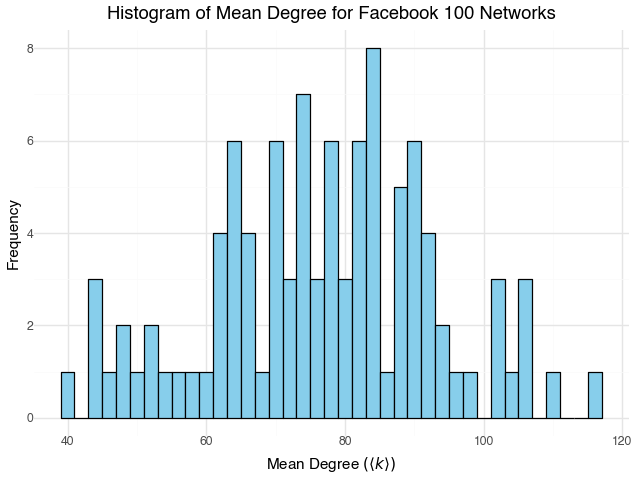
\includegraphics[width=0.95\textwidth]{../figures/mean_degree_histogram.png}
    \caption{Mean degree histogram for the Facebook network of 100 schools.}
    \label{fig:histogram_fb100}
\end{figure}

\subsection*{Part B}

\[
\langle k_v \rangle = \frac{1}{2m}\sum_{u=1}^n \sum_{v=1}^n A_{uv} k_v
\]

Using $m = \frac{n\langle k \rangle}{2}$ and $k_v = \sum_{u=1}^n A_{uv}$:

\[
\langle k_v \rangle = \frac{1}{n\langle k \rangle} \sum_{u=1}^n \sum_{v=1}^n A_{uv} k_v = \frac{1}{n\langle k \rangle} \sum_{u=1}^n k_u^2
\]

Since $\langle k^2 \rangle = \frac{1}{n} \sum_{u=1}^n k_u^2$:

\[
\langle k_v \rangle = \frac{\langle k^2 \rangle}{\langle k \rangle}
\]

\begin{flushright}
\(
\blacksquare
\)
\end{flushright}

\subsection*{Part C}

\begin{figure}[t]
    \centering
    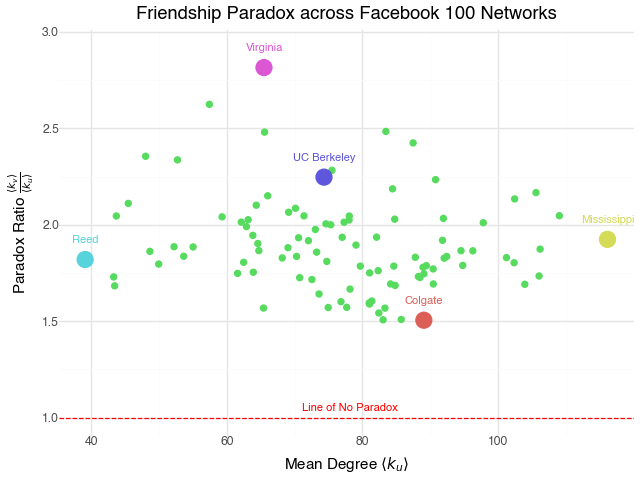
\includegraphics[width=0.95\textwidth]{../figures/paradox_ratio_plot.png}
    \caption{Friendship paradox analysis for Facebook networks of 100 universities. The x-axis shows mean degree, and the y-axis shows the ratio of neighbors' mean degree to the node's mean degree. The red dashed line at $y=1$ marks no friendship paradox. Highlighted points represent five universities: Reed, Colgate, Mississippi, Virginia, and UC Berkeley.}
    \label{fig:scatterplot_friendship_paradox}
\end{figure}

(i) The friendship paradox is clearly observed across these networks. Figure \ref{fig:scatterplot_friendship_paradox} shows that all universities have a paradox ratio $\frac{\langle k_v \rangle}{\langle k_u \rangle} > 1$, indicating nodes' friends consistently have more connections than the nodes themselves. 

\begin{itemize}
    \item Reed: Lowest mean degree with moderate paradox ratio
    \item Colgate: Slightly above-average mean degree with lowest paradox ratio
    \item Virginia: Below-average mean degree with highest paradox ratio
    \item UC Berkeley: Average mean degree with slightly above-average paradox ratio
    \item Mississippi: Highest mean degree with average paradox ratio
\end{itemize}

\noindent (ii) There is a positive relationship between the paradox ratio and network mean degree. As shown in the figure \ref{fig:scatterplot_friendship_paradox}, the friendship paradox becomes more pronounced in networks with higher mean degrees. This suggests that in more connected networks, nodes with more friends are likely to have even more highly connected friends, increasing the friendship paradox effect.\\

\noindent The friendship paradox emerges from the statistical bias in network degree distributions. In real-world social networks, high-degree nodes (individuals with many connections) are disproportionately represented in neighbor lists. When randomly selecting a node's neighbor, you're more likely to choose a neighbor from a highly connected individual. This mathematical property means that, on average, a person's friends will have more connections than the person themselves. Formally, this is represented by the inequality $\langle k_v \rangle = \frac{\langle k^2 \rangle}{\langle k \rangle} > \langle k \rangle$, which indicates that the mean neighbor degree is always greater than the network's average degree when connection variance exists.

\subsection*{Part D}

The majority illusion in social networks occurs when a trait that is rare in the overall population appears to be common from most individuals' perspectives. While the global fraction of nodes with the trait is less than half ($q = \frac{1}{n}\sum_u x_u < 0.5$), the fraction of neighbors with the trait exceeds half ($\langle x_v \rangle > 0.5$). This phenomenon emerges when nodes with the trait tend to have high degrees, similar to the friendship paradox. The illusion arises because while the global fraction $q$ weights all nodes equally, the neighbor average $\langle x_v \rangle$ is weighted by node degrees $k_v$, causing high-degree nodes to have disproportionate influence on local observations.

\subsection*{Part E}

\begin{figure}[t]
    \centering
    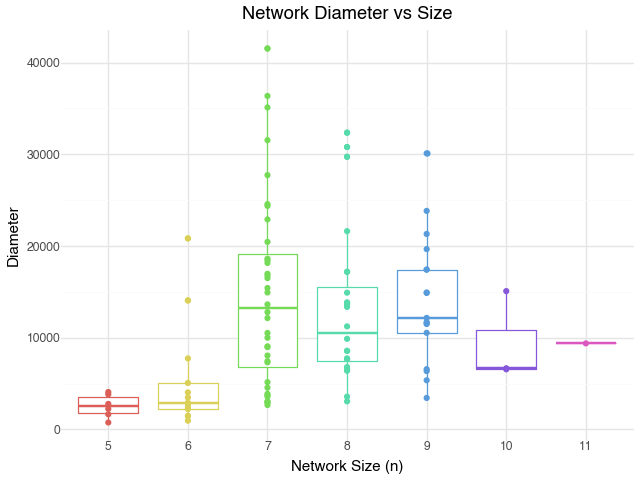
\includegraphics[width=0.95\textwidth]{../figures/diameter_vs_size.png}
    \caption{Network diameter vs. size for the Facebook network of 100 universities. The x-axis shows network size, and the y-axis shows network diameter. Histograms display the distributions, with points overlaid for reference. }
    \label{fig:diameter_vs_size}
\end{figure}

\begin{figure}[t]
    \centering
    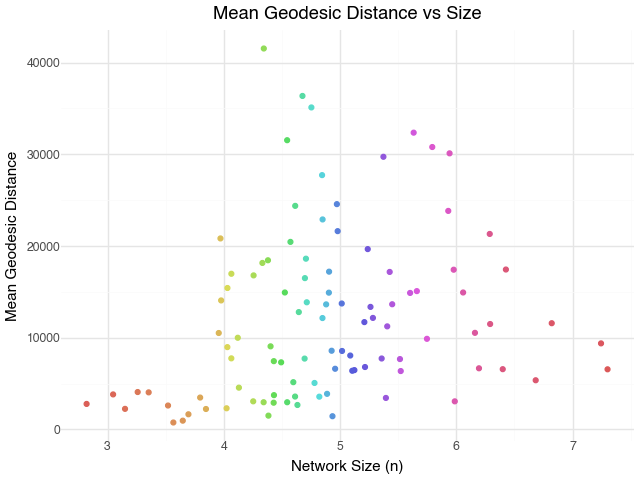
\includegraphics[width=0.95\textwidth]{../figures/mean_geodesic_distance_vs_size.png}
    \caption{Scatterplot of Mean geodesic distance vs. network size for the Facebook network of 100 universities. The x-axis shows the network size, while the y-axis represents the mean geodesic distance. Colors indicate nothing important and is meerly included for visual effects. }
    \label{fig:mean_geodesic_distance_vs_size}
\end{figure}
The mean geodesic distance is the average shortest path between node pairs. As shown in Figure \ref{fig:mean_geodesic_distance_vs_size}, it grows with network size, supporting the "six degrees of separation" concept, where connections remain short even in large networks.\\

\noindent The network diameter is the longest shortest path between nodes. Figure \ref{fig:diameter_vs_size} suggests the diameter of modern Facebook networks is smaller than in 2005 due to increased density and connectivity, consistent with the small-world phenomenon.\\

\noindent Both figures support the idea that social networks are highly interconnected, keeping path lengths short despite their size.
\section*{Problem 6}

I read the paper ``Private Traits and Attributes Are Predictable from Digital Records of Human Behavior" by Kosinski et al. The paper focuses on how simple digital records of human behavior, like Facebook Likes, can predict private and sensitive traits. The main goal was to figure out how accurate these predictions could be and to think about what this means for privacy and how personal data can be used.\\

\noindent The main question they were trying to answer was: Can Facebook Likes predict human attributes such as sexual orientation, political views, intelligence, life satisfaction, and more? The researchers worked with data from over 58,000 people, including their Facebook Likes, personality test results, and demographic information. They used methods like logistic regression to predict categorical traits and linear regression for continuous traits. They also applied dimensionality reduction and cross-validation to make sure their models were reliable.\\

\noindent The authors did a lot of things really well. First, they had a big sample size, which makes their results more robust. They also kept the models simple and easy to understand, which is great because it helps make the findings clearer. Another thing they did well was showing how this kind of prediction could be both helpful and risky—for example, predicting someone's pregnancy or political beliefs just based on their Likes. They didn't just explain it theoretically; they actually demonstrated how much information could be pulled from just a few clicks.\\

\noindent That said, there were a few areas where they could've done better. Even though they mentioned privacy concerns, they didn't dig into some key issues, like how their model could overfit or how biases in the data might mess with the results. For example, not everyone uses Facebook the same way, so their findings might not apply universally. They also didn't really explain what steps they took (if any) to deal with those biases. Lastly, they could've talked more about the ethical implications of using this kind of predictive technology, like how it could harm people if the information is used unfairly or incorrectly.\\

\noindent If I were to suggest some future directions, I think it would be interesting to look at how traits change over time. For example, could exposure to certain types of content shift someone's political views or life satisfaction? Another idea is to figure out the minimum amount of data needed to make accurate predictions—like how many Likes, search queries, or other digital footprints are enough to reliably predict traits. It would also be interesting to apply this to other data sources, like streaming habits or search history, to see if the results hold up across different platforms.

\end{document}